\section{Experiments}

It is now time to investigate, how the two efficient algorithms that
we derived in the previous section behave on real world datasets,
both in the context of maximum likelihood estimation as well as
in a Bayesian setting.
In order to do so, we selected three benchmark datasets in advance
that will be used to compare both algorithms to each other as
well as to the baseline uniform sampling procedure, where each
sample is simply selected with equal probability.

It is important to emphasize, that the datasets used in the evaluation
are not a result of cherry picking: We selected the same datasets
as \cite{on-coresets} as well as \cite{coresets-strengthened}
in order to be comparable to other works in the field, without
testing in advance if our algorithms look good on them or not.

Finally, we note that all of the following experiments were
implemented in Python and executed on an
AMD Ryzen 7 2700x processor with 8 cores of 3.7GHz clock speed
and 16GB of RAM.
The code for all the experiments is open source and can be
found publicly accessible on Github.\footnote{
    \url{https://github.com/cxan96/efficient-probit-regression}
}

\subsection{Datasets}

The datasets that are used in the empirical evaluation of our
algorithms are called Covertype\footnote{
    \url{https://archive.ics.uci.edu/ml/datasets/Covertype}
}, Kddcup\footnote{
    \url{https://kdd.ics.uci.edu/databases/kddcup99/kddcup99.html}
} and Webspam\footnote{
    \url{https://www.csie.ntu.edu.tw/\~cjlin/libsvmtools/datasets/binary.html\#webspam}
} and are
all publicly available.

The Covertype dataset consists of $n=581012$ observations of 30x30m
forest patches of wilderness areas located in the
Roosevelt National Forest of Northern Colorado, USA.
The task is to predict the so called covertype of each of these
patches, i.e. the dominant tree species, based on $d=54$
observed features. There are seven distinct tree species that
appear in the dataset, so we have a multiclass problem. To transform
the problem into a binary classification problem that can be
subjected to a probit analysis, we adapted the task to distinguish the
tree species "Lodgepole Pine" from the other six species, thus
obtaining a balanced problem of $49\%$ positive vs $51\%$ negative
observations.
As an additional preprocessing step, all continuous features of the
dataset were scaled to have a mean of zero as well as unit variance.
In addition, an intercept column of all ones was appended to the data.

The Webspam datasets consists of $n=350000$ observations of
web pages, that can either be classified as spam or no spam, based
on the occurence of 254 distinct words on the web page.
$61\%$ of the observations in the dataset are labeled as spam
and the other $39\%$ are labeled as no spam. The task is to predict,
whether a given web page is spam or not.
The features consist of binary $0/1$ observations that indicate, if
a given word is present on a web page or not.
In a preprocessing step, words that are never present
in the dataset were removed, as well
as words that are only present on a single web page.
After preprocessing, the dataset that is subjected to the
experiments consists of $d=128$ binary features.
An intercept column of all ones was appended to the Webspam dataset
as well.

The Kddcup dataset consists of $n=494021$ observations of network
connections, where the task is to predict if a connection is
"good" or "bad", i.e. to distinguish, whether a hacker tried
to gain unauthorized
access to a network or whether someone tried to establish a
normal and authorized connection.
$80\%$ of the connections in the dataset are "bad" and the other
$20\%$ are "good" connections.
In a preprocessing step, $d=33$ continuous features
were retained from the data and scaled to a mean of zero and
unit variance. Just like the other datasets, an intercept column
of all ones was appended to the Kddcup data as well.

\subsubsection{A Visual Comparison of the Datasets}

Before we evaluate the three competing algorithms on each of
the datasets, we first make an attempt at uncovering some of
the structural characteristics of the data, that could
potentially help us to learn more about the situations in which
the algorithms perform well or might fail.

In order to do so, we first project each dataset onto
its first two principal components, which where obtained
as a result of a principal component analysis
\cite{principal-components}.
The first two principal components are orthogonal vectors that
represent the two directions of the data,
in which the highest variance occurs.
By projecting each datapoint onto the subspace spanned by
the first two principal components, we have
a way of visualizing the datasets in a two dimensional space, while
still retaining as much variance as possible, even though we are
reducing the dimensionality to only 2.

Next, we draw two distinct samples from the reduced datapoints,
each consisting of 500 points. The first one is a uniform sample,
where each datapoint is sampled with equal probability.
The second sample is drawn with probabilities that are proportional
to the statistical leverage scores of the observations with
respect to the original dataset, without applying a PCA.
Both of these samples are presented for each of the datasets in
figure~\ref{fig:dataset-comparison}.

\begin{figure}[ht!]
    \centering
    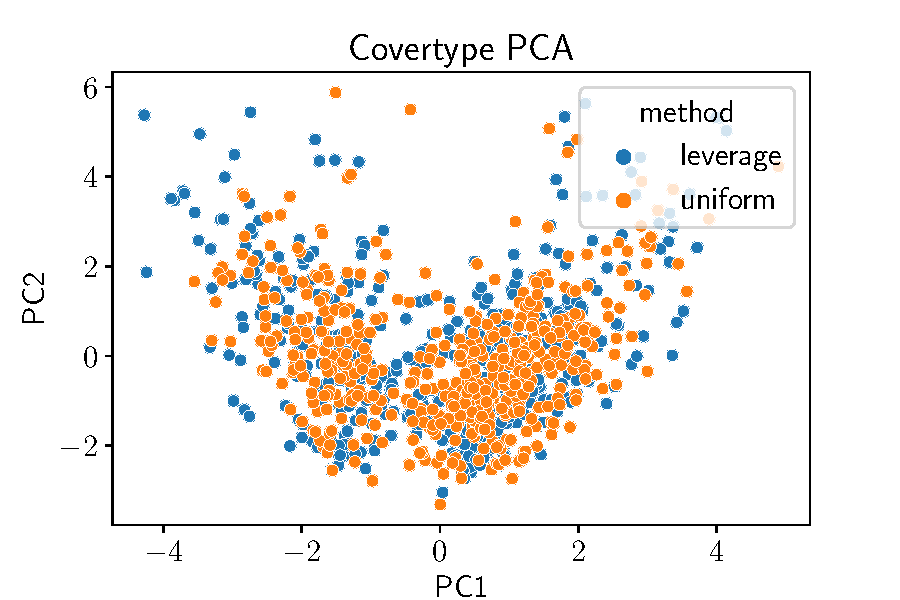
\includegraphics[width=.49\linewidth]{figures/covertype_pca.pdf}
    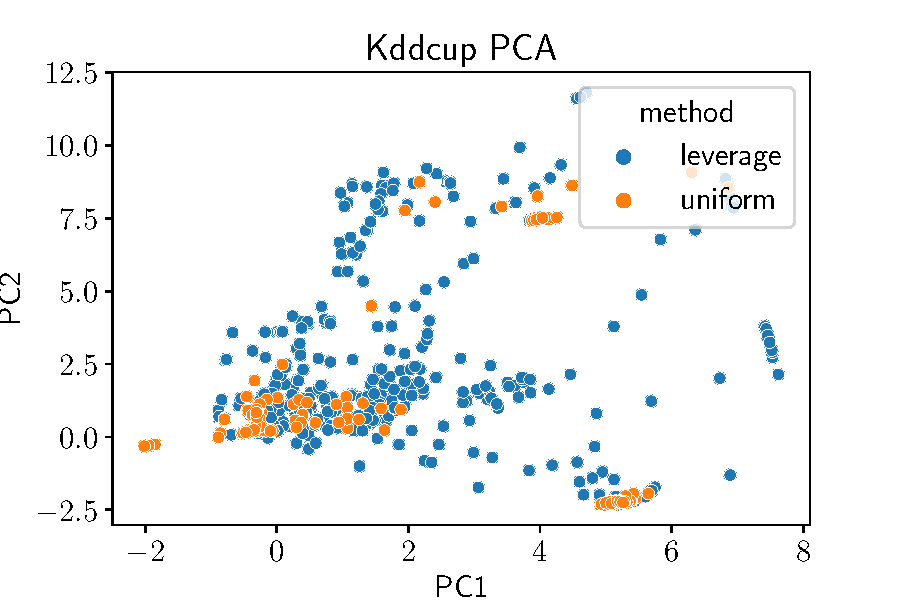
\includegraphics[width=.49\linewidth]{figures/kddcup_pca.pdf}
    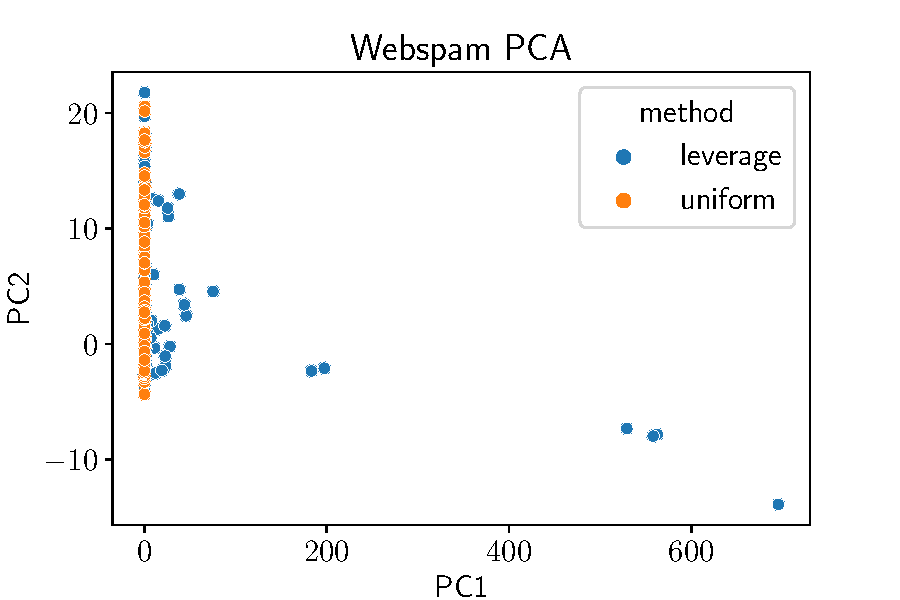
\includegraphics[width=.49\linewidth]{figures/webspam_pca.pdf}
    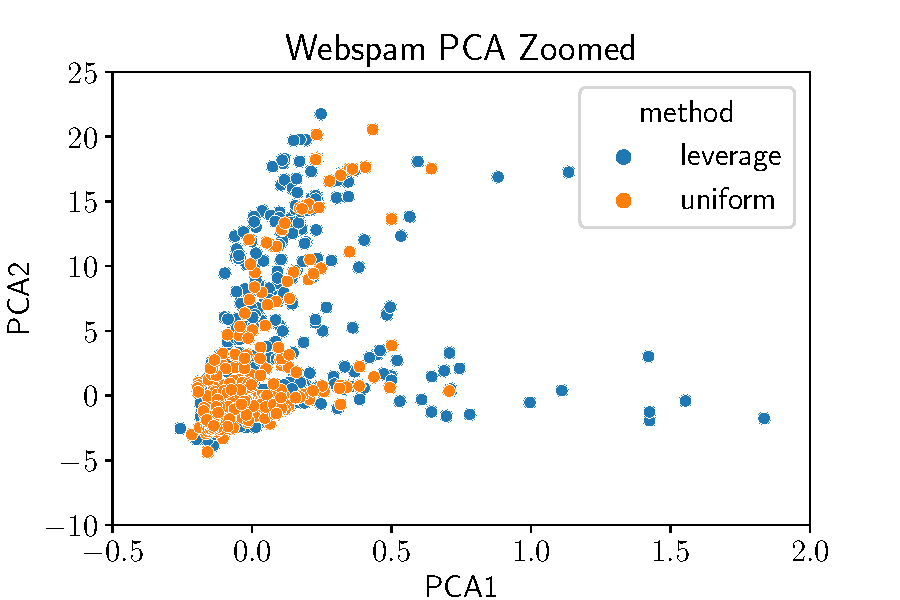
\includegraphics[width=.49\linewidth]{figures/webspam_pca_zoomed.pdf}
    \caption{The datasets are compared by projecting the datapoints
        onto the first two principal components and then drawing
        a random sample of 500 points (a) uniformly and (b) proportionally to the
        statistical leverage scores of the original data.}
    \label{fig:dataset-comparison}
\end{figure}

We can see, that the samples reveal some interesting characteristics
of the datasets. Starting with Covertype, we notice that there
hardly seems to be any difference between the uniform sample and
the leverage score sample. Taking into consideration, that the
statistical leverage scores assign a higher importance to
outliers or "unusual" datapoints, we can conclude that there don't
seem to be too many unusual observations within the Covertype
dataset, or else the two samples would differ more substantially.
It seems to be the case, that a uniform sample is already
sufficient to capture most of the inherent structure of the data,
without having to put extra weight on unusual datapoints, which
simply appear not to exist in this dataset.
Thus, from now on, it seems reasonable to think of the
Covertype dataset as being
a representative for such situations, where the data is
already quite uniformly distributed and not a lot of outliers are
present, i.e. where a uniform sample already seems to
yield good results.

In contrast to Covertype, the Kddcup dataset exhibits a different
picture. Here, we can see that the uniform sample and the leverage
score sample differ way more substantially than it was the case
for the Covertype dataset.
While the uniform sample only seems to occupy a very limited portion
of the feature space, most of it being a cluster of
many points close to the origin,
the leverage score sample covers a lot more
of the feature space,
indicating that there are a variety of unusual datapoints,
or outliers present,
which the uniform sample misses.
Thus, it seems that we can think of the Kddcup dataset as an
example of a situation,
where on the one hand, we have a lot of similar observations that
are concentrated within a comparatively small proportion of
the feature space, but on the other hand, we also have a
considerable amount of unique observations, which are scattered
around the feature space
while seemingly not belonging to any particular cluster.

Lastly, another interesting situation is presented to us when taking
a look at the two samples of the Webspam dataset.
What strikes the eye first, is that there seem to be some truly
extreme outliers present in the dataset, that the leverage score
sampling picked up on. Only by zooming in on the more crowded area
of the feature space and thereby ignoring those extreme outliers,
we can see the remaining parts of the two samples, which seem to
be rather similar, just like in the situation of the Covertype dataset.
It thus seems to be the case, that the Webspam dataset is an example
of a situation, where on the one hand, the vast majority of the
datapoints are concentrated around some region of the feature space,
but on the other hand, there are also a few hard hitting outliers present,
which exhibit enormous differences to the majority of the other
observations.

\subsection{Coreset-Based Maximum Likelihood Estimation}

We are now ready to investigate, how well our three algorithms
(two pass coreset construction, online coreset construction and
uniform sampling) perform at the task of data reduction
with the goal of estimating the
parameter vector of a probit model on the three datasets that
we just introduced via maximum likelihood estimation.
In order to do so, we present the following experimental setup:

For each of the datasets, we first obtain the objective function
$f(\beta)$ of the original optimization problem without applying
any data reduction and then solve the problem to find the
unique solution $\beta^{opt}$.
Next, we apply our data reduction algorithms in order to select
a small subset of the original data, yielding the reduced
objective function $\tilde{f}(\beta)$. We solve this
smaller optimization problem in order to obtain the solution
$\tilde{\beta}$. Our goal is to see, if the solution on the
reduced dataset, $\tilde{\beta}$, is also a good solution
for the original problem. In order to evaluate the approximation
quality, we compute what we call the approximation ratio:
\begin{equation*}
    \operatorname{approximation\ ratio} = \frac{f(\tilde{\beta})}{f(\beta^{opt})},
\end{equation*}
which always evaluates to a real number in the interval $[1, \infty)$.
The closer this value is to $1$, the better is the quality of
the approximation.

We run this procedure for each algorithm on each of the datasets
for multiple different reduction sizes. Because the algorithms
are not deterministic, we ran each of the experiments a total
of 51 times. The resulting medians as well as the normalized
inter quartile range can be seen in figure~\ref{fig:ratio-plots}.

\begin{figure}[ht!]
    \centering
    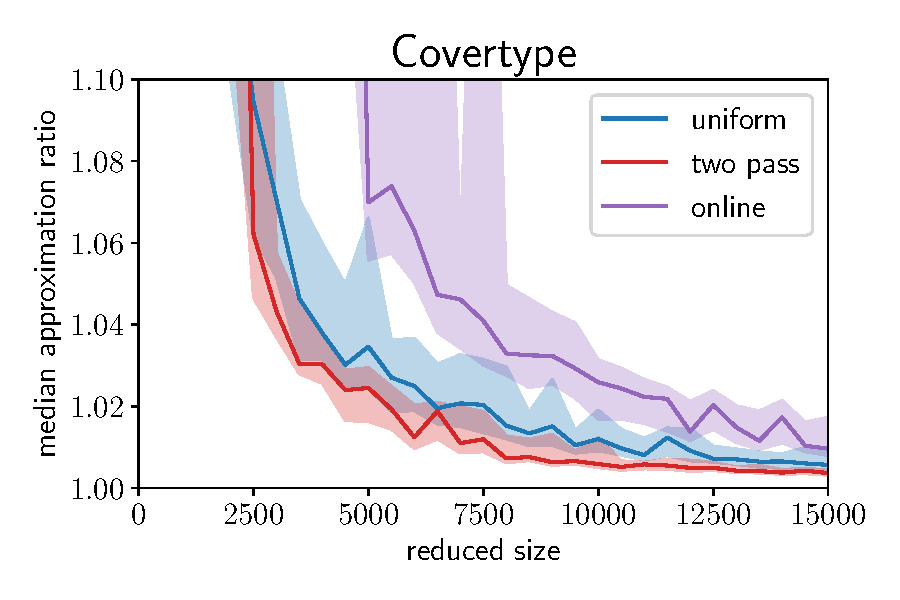
\includegraphics[width=.49\linewidth]{figures/covertype_ratio_plot.pdf}
    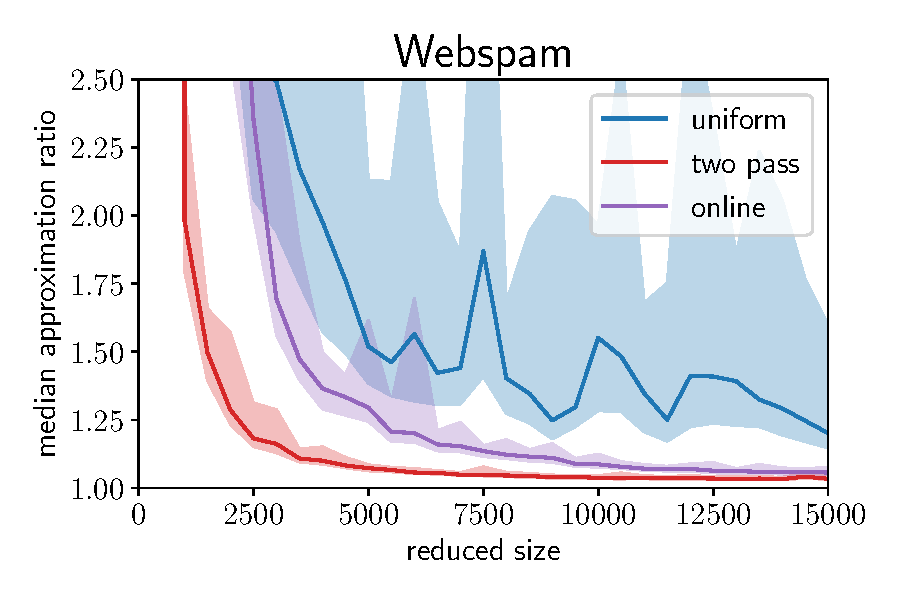
\includegraphics[width=.49\linewidth]{figures/webspam_ratio_plot.pdf}
    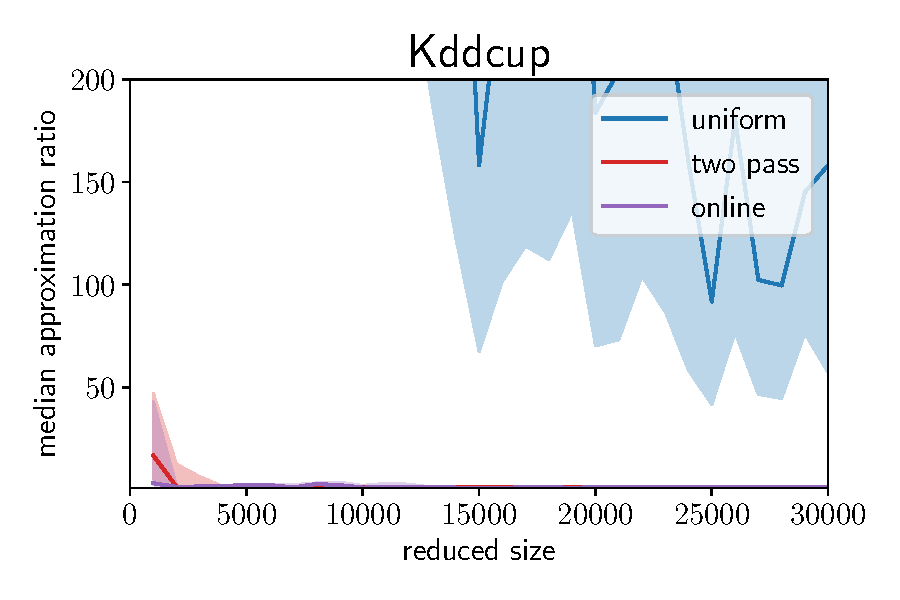
\includegraphics[width=.49\linewidth]{figures/kddcup_ratio_plot.pdf}
    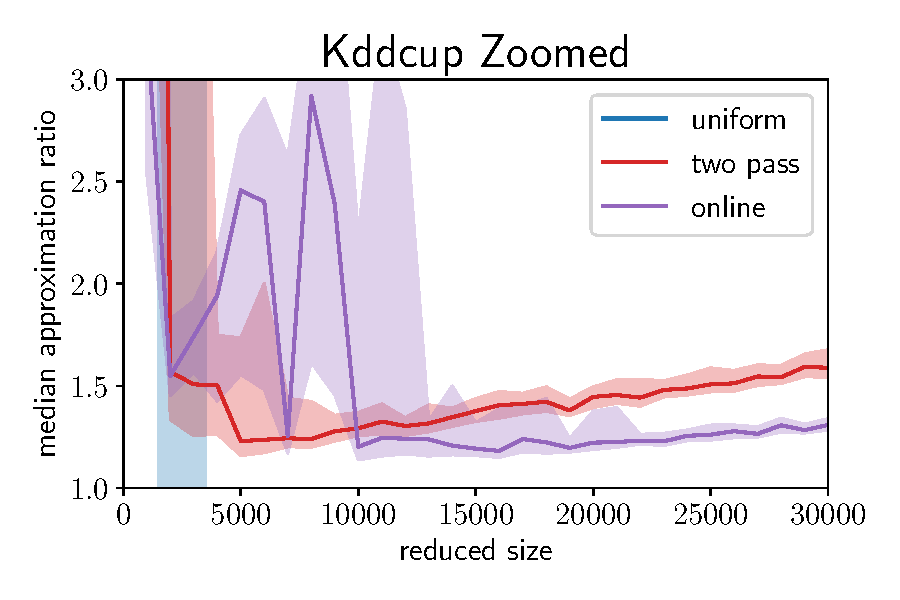
\includegraphics[width=.49\linewidth]{figures/kddcup_ratio_plot_zoomed.pdf}
    \caption{The medians as well as the normalized inter quartile
        ranges of the approximation ratios of the three
        algorithms uniform sampling, two pass coreset construction and
        online coreset construction on the datasets Covertype, Webspam
        and Kddcup for different data reduction sizes.
        For each reduction size, the experiments were repeated a
        total of 51 times.}
    \label{fig:ratio-plots}
\end{figure}

\subsubsection{Comparison of Approximation Quality}

Starting with the Covertype dataset, we can see that each algorithm
quickly reaches good approximation ratios of less than $1.02$
for subset sizes of only $15000$ datapoints, which are less than
$3\%$ of the original dataset.
Both, the uniform sampling as well as the two pass algorithm, are
close to each other in terms of approximation quality, although
the median ratio of the two pass algorithm is always better than
that of uniform sampling. The online algorithm performs worse than
the two competing algorithms, but it also quickly reaches a low
approximation ratio of less than $1.02$.
Interestingly, the fact that the results of our three algorithms
don't differ much on the Covertype dataset, could
be explained by our earlier
findings regarding the characteristics of the data.
For the Covertype dataset, we found that it could be a representative for
those situations, where the datapoints are already
quite homogeneously distributed, i.e. there
are not a lot of outliers, heavy hitters or other unusual points to worry
about and thus, a uniform sample can already be sufficient to
capture the relevant characteristics of the data.
Nevertheless, our two pass algorithm still outperformed the uniform
sampling procedure, albeit by only a small margin.

For the Webspam dataset, the picture looks a lot different. Here,
we can see for the first time that the uniform sampling algorithm
fails, while the two pass algorithm as well as the one pass
algorithms quickly reach low approximation ratios. On top of that,
the approximation ratios of the uniform sampling algorithm
exhibit a much higher degree of variation and thereby show a lot
less stability than the competing algorithms two pass and online.
Again, it is interesting to note, that these results could also
potentially be explained by our earlier observations:
When visualizing the Webspam dataset by using the first two
principal components, we already noticed that there are a few
extreme outliers present in the data. We also noticed, that
the uniform sample was unable to pick up on those outliers
and only concentrated on the bulk of the datapoints in
the center of the feature space. Now, in our
maximum likelihood experiments,
we can see that the uniform sampling procedure also
exhibits major weaknesses
for the Webspam dataset. It thus seems reasonable to assume,
that this is again happening because the uniform sampling
algorithm misses the extreme outliers, which could potentially have a
high impact on the objective function.
Both, the two pass algorithm as well as the online algorithm,
don't miss those important points thanks to their more
adaptive importance sampling distributions that also take
the statistical leverage scores into account, and therefore show a
stable convergence behavior towards low approximation rates.

The most dramatic differences between uniform sampling and the
competing algorithms can be observed when looking
at the results for the Kddcup dataset. Here, we can see that
uniform sampling fails terribly and doesn't even reach
approximation ratios lower than $50$. When zooming in, we can
see that our other two algorithms perform much better, although they
also seem to show some difficulties. It is especially interesting
to note, that the online algorithm seems to perform better than the
two pass algorithm, even though its approximations of the
statistical leverage scores are less accurate.
Together with our earlier observations of the structure of the
Kddcup dataset, it seems that Kddcup is a particularly difficult
dataset to compress. Even though the sampling methods that
also rely on the leverage scores clearly outperform the
uniform sampling algorithm, they also show difficulties with
regard to convergence. We should also note here, that the
maximum size of $30000$ points for the Kddcup dataset already
takes up more than $6\%$ of the whole dataset, which is more than
double as much as what was needed for the Covertype dataset to
achieve a much better approximation quality.
Thus, the Kddcup dataset seems to be more challenging for all the
competing algorithms, although the two pass algorithm and the
online algorithm handle the difficult conditions way better than
the uniform sampling algorithm.

\subsubsection{Comparison of Running Times}

We round off our first experiment with a discussion regarding the
runtimes of the algorithms compared to the time it takes to
solve the original problem without prior reduction, as well as
a discussion of the tradeoffs between approximation quality and
running time.

It must be noted, that the online coreset algorithm
had to be excluded from the comparison due to its
incomparably high running time of $O(nd^2)$, which would have
made it impossible to execute a sufficient number of experiments.
However, we remark that the advantage of the online algorithm isn't
necessarily its speed, but that it is able to construct coresets
even when two passes over the data are impossible and every sampling
decision has to be made immediately. Also, it might be possible
to drastically increase the efficiency of the online algorithm,
by running mutiple parallel instances of it on a distributed
cluster and then equally balancing the load of the incoming
data records between
each of the instances, but these possible adaptations are
left open for future work.

The total running times for obtaining the maximum
likelihood estimate of the probit model for each of the
datasets without applying any data reduction are given in
table~\ref{tab:running-times} and will serve as a
baseline for further discussions.

\begin{table*}[ht!]
    \centering
    \begin{tabular}{ l | l| l| l}
        \hline
                           & \textbf{Covertype} & \textbf{Kddcup} & \textbf{Webspam} \\ \hline
        Total running time & $535$ seconds      & $103$ seconds   & $447$ seconds    \\ \hline
    \end{tabular}
    \caption{The total running times that it takes to obtain the maximum
        likelihood estimator for each of the datasets.}
    \label{tab:running-times}
\end{table*}

In figure~\ref{fig:runtime-plots}, we present the
tradeoffs between approximation ratio and running time
for uniform sampling as well as for the fast two pass algorithm.
The reported times include the data reduction step as
well as the optimization step, in order to be able to
compare the times to the total running times without data reduction.

\begin{figure}[t]
    \centering
    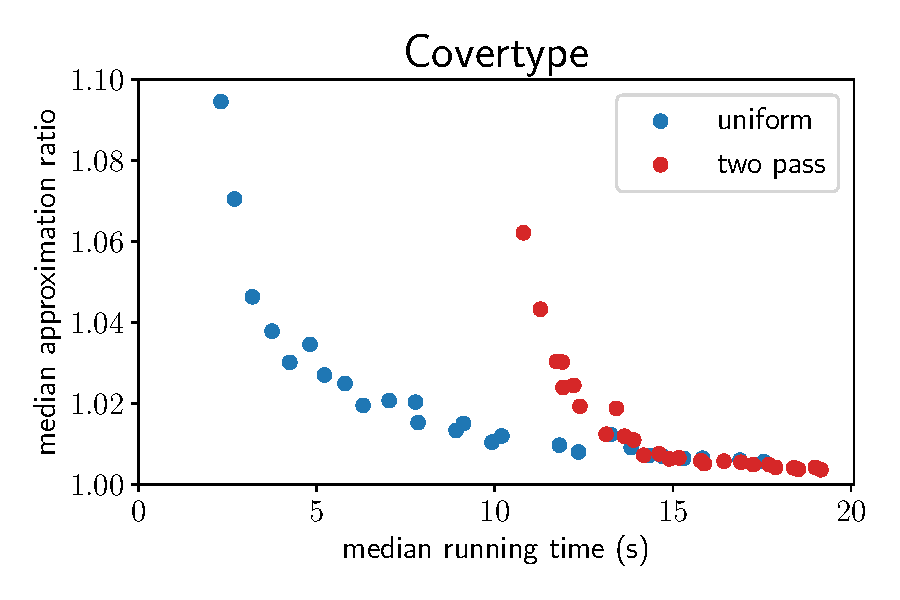
\includegraphics[width=.49\linewidth]{figures/covertype_runtime_plot.pdf}
    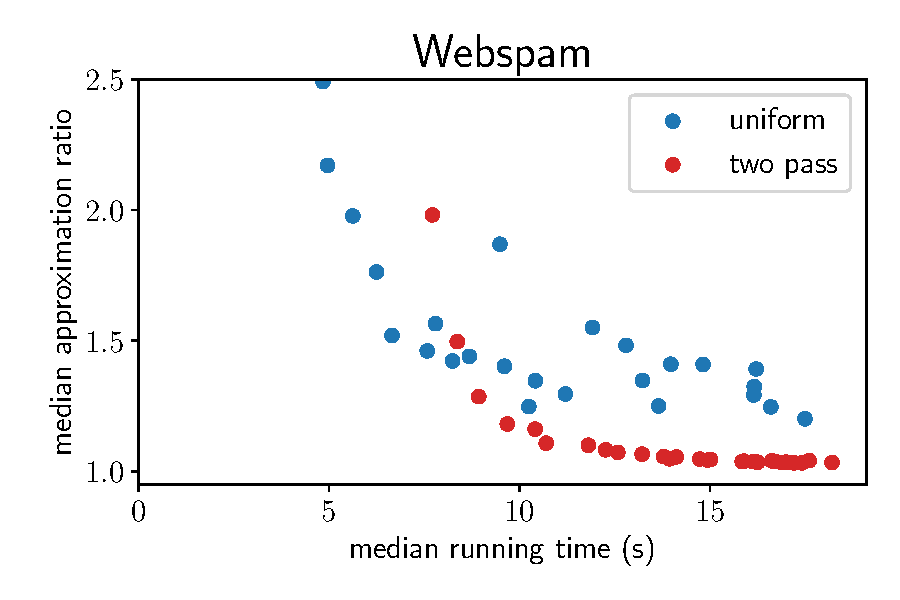
\includegraphics[width=.49\linewidth]{figures/webspam_runtime_plot.pdf}
    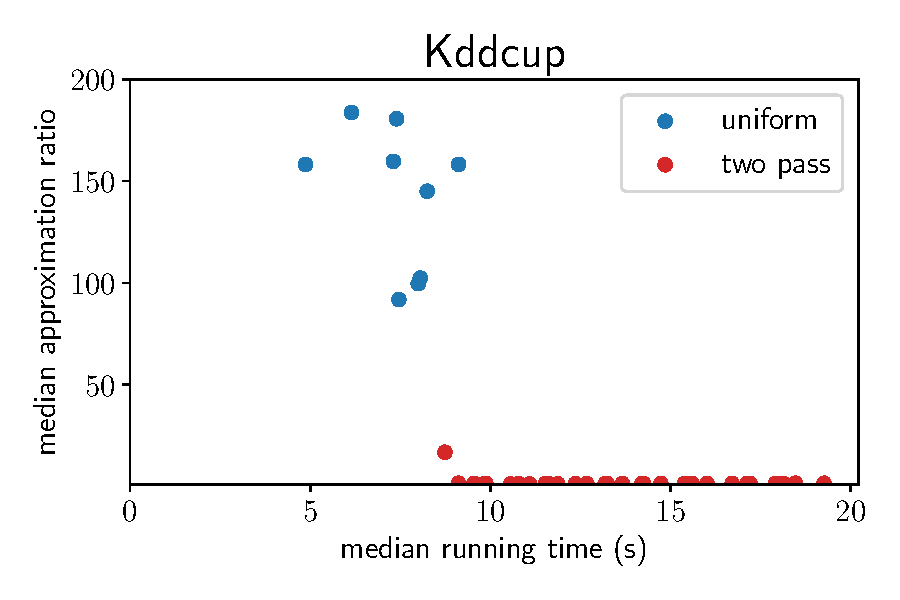
\includegraphics[width=.49\linewidth]{figures/kddcup_runtime_plot.pdf}
    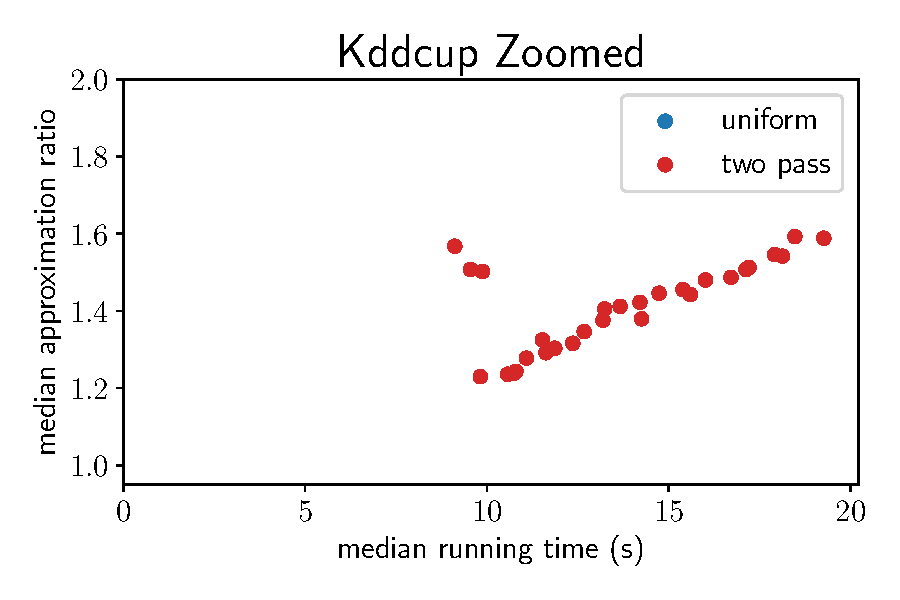
\includegraphics[width=.49\linewidth]{figures/kddcup_runtime_plot_zoomed.pdf}
    \caption{The plots show the tradeoffs between running time and
        approximation ratio for the uniform sampling algorithm and the
        fast two pass algorithm on our datasets.
        Every point represents the median in running time, as well
        as the median in approximation ratio, for a given
        data reduction size.
    }
    \label{fig:runtime-plots}
\end{figure}

When looking at the results for the Covertype dataset, we can see
that the uniform sampling algorithm outperforms the two pass
algorithm in terms of speed, but is unable to reach the same degree
of approximation quality as the two pass algorithm. The running times of
the uniform sampling procuedure range roughly between 1 and
10 seconds, but decent results are only achieved when investing
at least 5 seconds. On the other hand, the running times of the
two pass algorithm range between 10 and 20 seconds, thus taking
almost twice as long. But compared to the total running time
for the Covertype dataset without reduction, we can see that
even the two pass algorithm reduces the total running time
by more than $96\%$, from 535 seconds to less than 20 seconds.

Taking a look at the Webspam dataset, we can see an interesting
picture: Not only does the two pass algorithm show better
approximation rates than the uniform sampling algorithm, but
it also shows similar running times. Thus, for the Webspam dataset,
the two pass algorithm almost dominates the uniform sampling
in the two criterias, since it has similar running times but
achieves a better approximation quality.
For running times of 15 seconds, the fast two pass algorithm already
achieves decent results, thus we can say that the
original time for solving the unreduced problem was again reduced
by more than $96\%$, from 447 seconds to only 15 seconds.

In the case of Kddcup, the comparison is almost pointless, because
the uniform sampling fails. We only include these results to show
that the running times of the two pass algorithm consistently
range between 10 and 20 seconds, even when the data is
substantially less well behaved, as we showed for the
Kddcup dataset. Here, the time savings are not quite as impressive
as for the Covertype and the Webspam dataset:
The total running time was "only" reduced by more than $80\%$,
from 103 seconds to less than 20 seconds. Still, we can
consider this a decent win, especially when keeping
in mind that the uniform sampling algorithm failed completely.

To conclude the discussion of our first experiment, we can
say that the slightly increased running time of the two
pass algorithm compared to the uniform sampling algorithm
should be of no concern, because the few seconds in excess
runtime were always well compensated by substantial
gains in approximation quality. For each dataset,
the two pass algorithm is able to reduce the total
optimization time by more than $80\%$, even $96\%$ for
the Covertype and for the Webspam dataset.

\subsection{Coreset-Based Bayesian Inference}

The goal of our second experiment is to investigate, if our
algorithms can be successfully applied as a data reduction
step to cut down the computational cost of performing
a full Bayesian probit analysis on our three datasets.
In order to do so, we use the efficient Gibbs sampler
described earlier in section~\ref{sec:gibbs} to generate
samples with and without a preceding data reduction step using
our algorithms, and see how they compare to each other.
But before we can get into the full experimental setup,
we must note that in order to use the Gibbs sampler together
with our algorithms, it has to be slightly adapted
to account for the sample weights that are an
essential component of our coreset algorithms,
which is briefly covered in the next section.

\subsubsection{Adapting the Gibbs Sampler for Weighted Coresets}
\label{sec:gibbs-adaptation}

\subsubsection{Experimental Setup}

We use a similar experimental setup
as in \cite{scalable-bayesian-logreg} and
\cite{bayesian-regression}:
First, we arbitrarily selected a relatively uninformative
prior distribution of
\begin{equation*}
    \beta \sim \mathcal{N}(0, 10 \cdot \mathcal{I}),
\end{equation*}
where $\mathcal{I}$ is the identity matrix.
Next, we used the Gibbs sampler
to generate a sample of the full posterior
distribution without applying any data reduction for each
of the three datasets.
Each of the three full posterior samples has a size of $10000$,
and for each of the datasets, a different
burn in value was selected. For Covertype, a burn in
of 200 was sufficient, 2000 was needed for Kddcup and 3000
for Webspam.
Next, we applied our algorithms to each of the datasets
for a variety of reduction sizes and ran the adapted version of
the Gibbs sampler (see section~\ref{sec:gibbs-adaptation} above)
on the reduced data, obtaining a posterior sample of size 1000
for each data reduction size. The burn in values for
the reduced samples were set to be
the same as for the original unreduced data.


\begin{figure}[t]
    \centering
    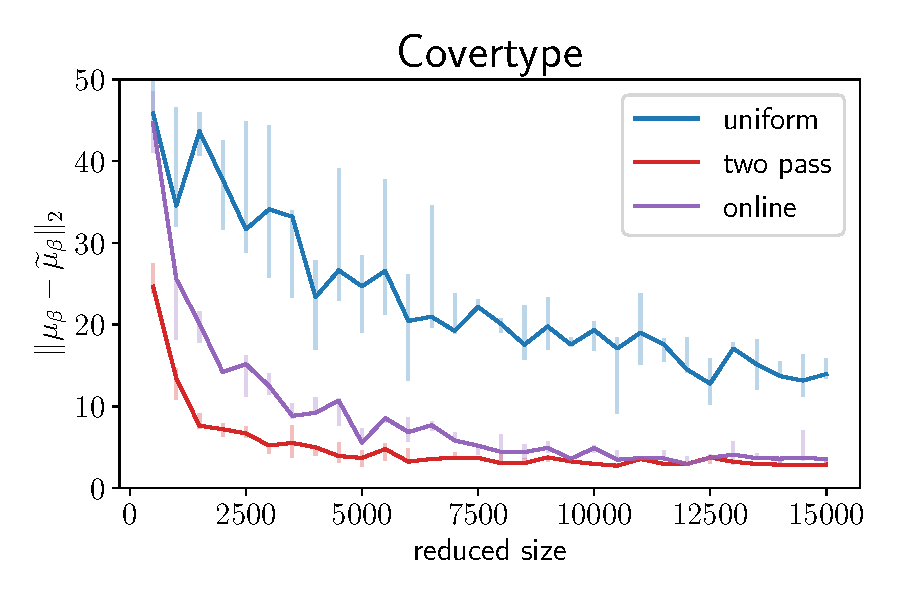
\includegraphics[width=.49\linewidth]{figures/covertype_bayes_plot_norm.pdf}
    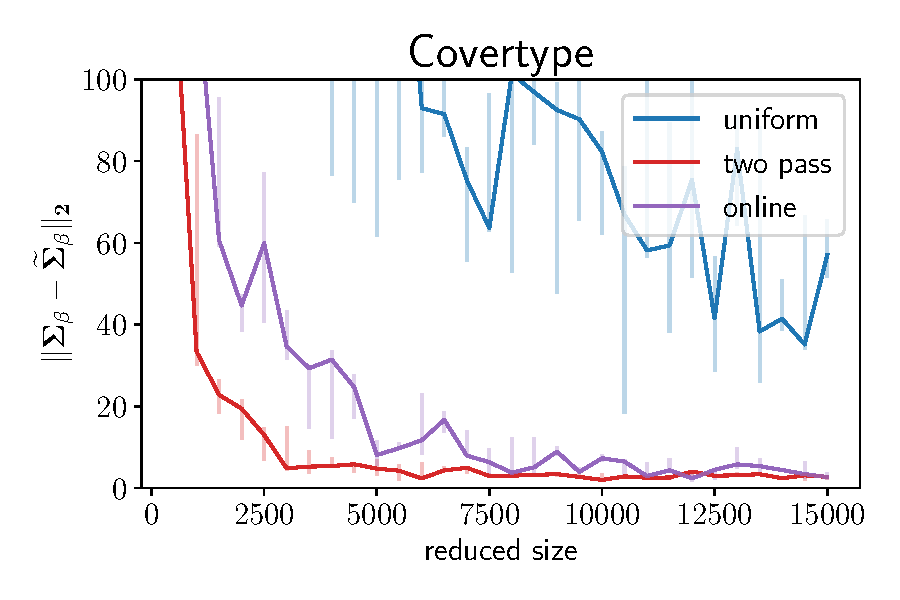
\includegraphics[width=.49\linewidth]{figures/covertype_bayes_plot_matrix_norm.pdf}
    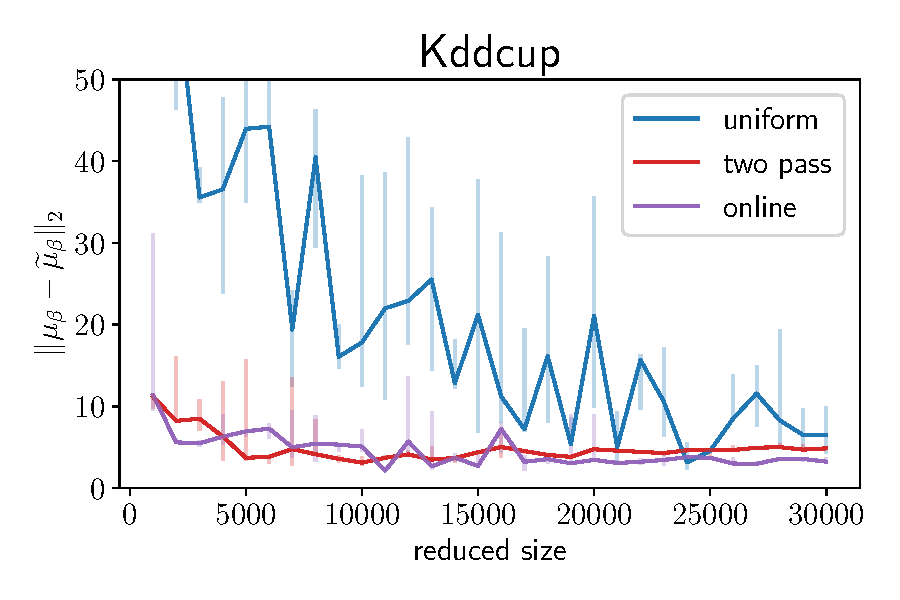
\includegraphics[width=.49\linewidth]{figures/kddcup_bayes_plot_norm.pdf}
    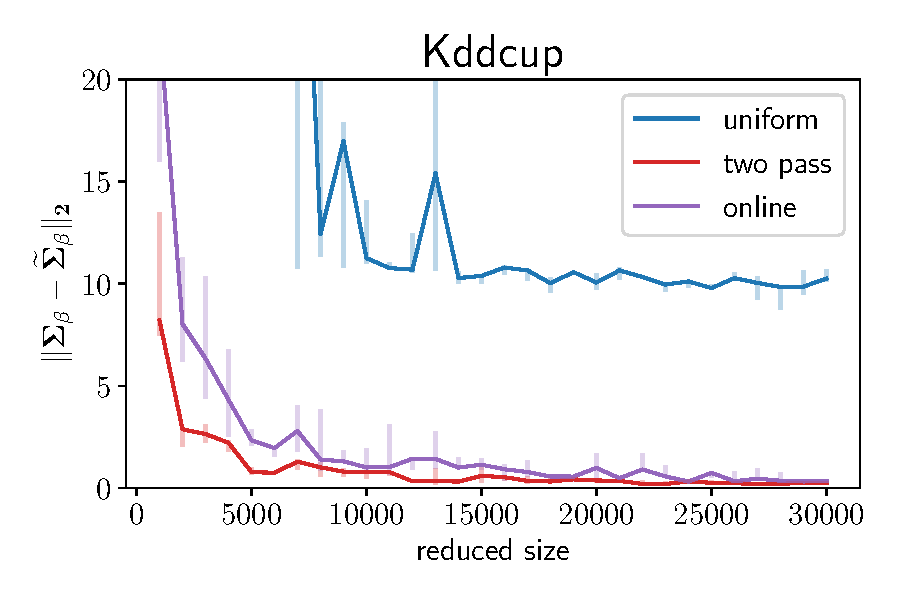
\includegraphics[width=.49\linewidth]{figures/kddcup_bayes_plot_matrix_norm.pdf}
    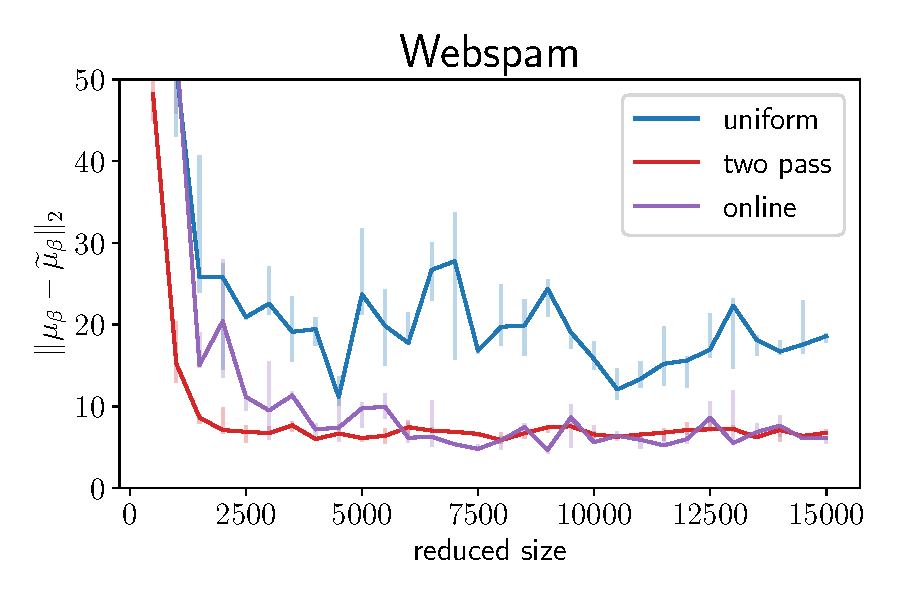
\includegraphics[width=.49\linewidth]{figures/webspam_bayes_plot_norm.pdf}
    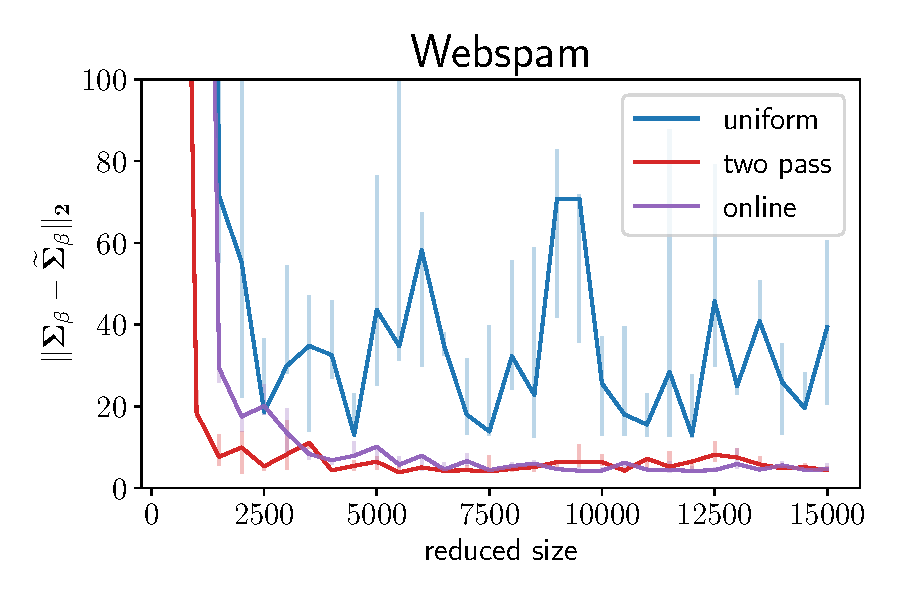
\includegraphics[width=.49\linewidth]{figures/webspam_bayes_plot_matrix_norm.pdf}
    \caption{TODO}
    \label{fig:bayes-plots-norm-cov}
\end{figure}

\begin{figure}[t]
    \centering
    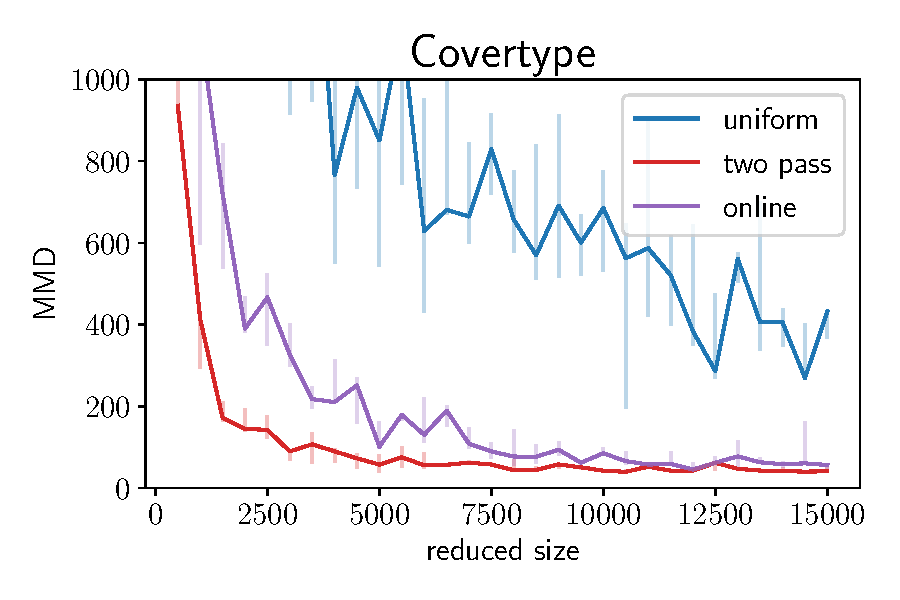
\includegraphics[width=.49\linewidth]{figures/covertype_bayes_plot_mmd.pdf}
    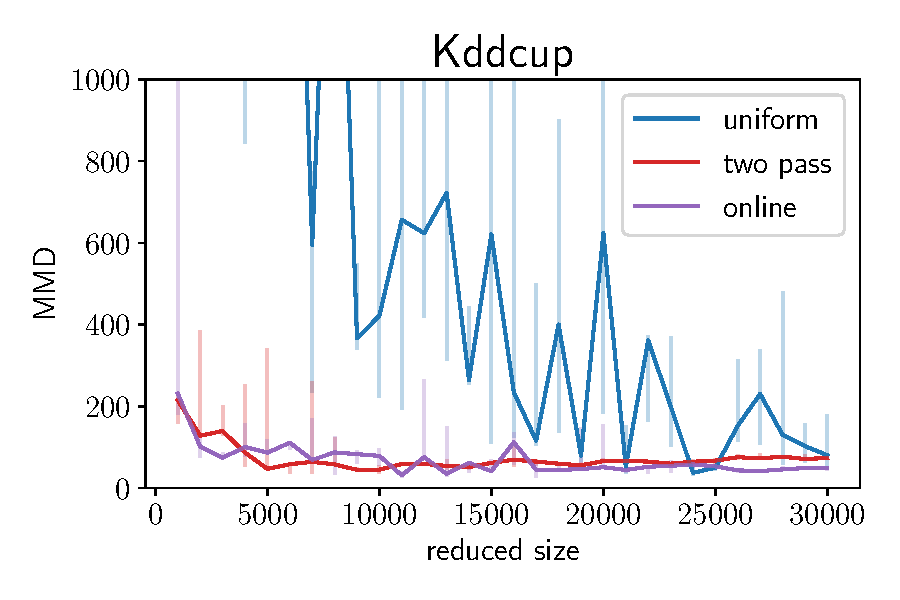
\includegraphics[width=.49\linewidth]{figures/kddcup_bayes_plot_mmd.pdf}
    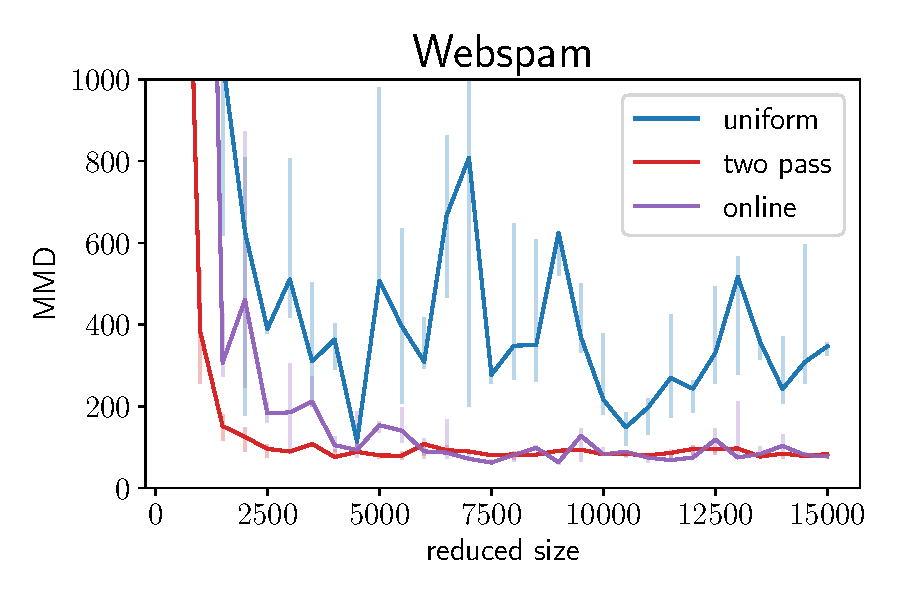
\includegraphics[width=.49\linewidth]{figures/webspam_bayes_plot_mmd.pdf}
    \caption{TODO}
    \label{fig:bayes-plots-mmd}
\end{figure}
